\documentclass[a4paper]{tufte-handout}

\usepackage{algorithm,algorithmic}
\usepackage{graphicx}
\usepackage{framed}
\usepackage{amsmath}
\usepackage[T1]{fontenc}
\usepackage{todonotes}
\usepackage{graphicx}
\hypersetup{
    colorlinks=true,
    linkcolor=blue,
    filecolor=magenta,      
    urlcolor=blue,
}

\title{Deep Learning Training Program}
\author{Sasank Chilamkurthy, Qure.ai}
\date{May 10, 2017}

\begin{document}
\maketitle
\tableofcontents

\section{Calculus: Recap}\label{calculus-recap}

Let's recap what a derivative is.

\subsection{Derivative}\label{derivative}

Derivative of function \(f(v)\) (\(f'(v)\) or \(\frac{df}{dv}\))
measures sensitivity of change in \(f(v)\) with respect of change in
\(v\).

\begin{marginfigure}
  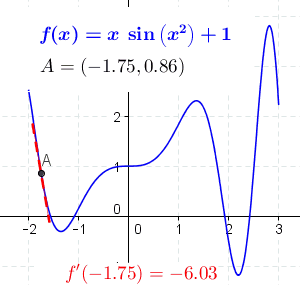
\includegraphics[height=50mm]{differential.png}
  \caption{Derivative illustration. Red is for positive \(v\)
direction and green is for negative \(v\) direction.
\href{https://en.wikipedia.org/wiki/Derivative}{Source}.}
\end{marginfigure}

Direction (i.e sign) of the derivative at a points gives the direction
of (greatest) increment of the function at that point.

\subsection{Gradient}\label{gradient}

The gradient is a multi-variable generalization of the derivative. It is
a vector valued function. For function \(f(v_1, v_2, \ldots, v_n)\),
gradient is a vector whose components are \(n\) partial derivatives of
\(f\):

\[ \nabla f = (\frac{\partial f}{\partial v_1 }, \frac{\partial f}{\partial v_2 }, \ldots, \frac{\partial f}{\partial v_n })\]


\begin{marginfigure}
  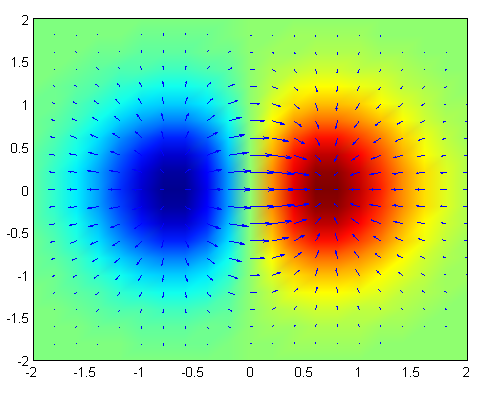
\includegraphics[height=50mm]{gradient.png}
  \caption{Gradient of the 2D function \(f(x, y) = xe^{−(x^2 + y^2)}\) is
plotted as blue arrows over the pseudocolor (red is for high values
while blue is for low values) plot of the function.
\href{https://en.wikipedia.org/wiki/Gradient}{Source}.}
\end{marginfigure}


Similar to derivative, direction of the gradient at a point is the
steepest ascent of the function starting from that point.

\section{Optimization}\label{optimization}

Given a function \(C(v_1, v_2, \ldots, v_n)\), how do we optimize it?
i.e, find a point which minimizes this function globally.

This is a very generic problem; lot of practical and theoretical
problems can be posed in this form. So, there is no general answer.

\subsection{Gradient Descent}\label{gradient-descent}

\begin{marginfigure}
  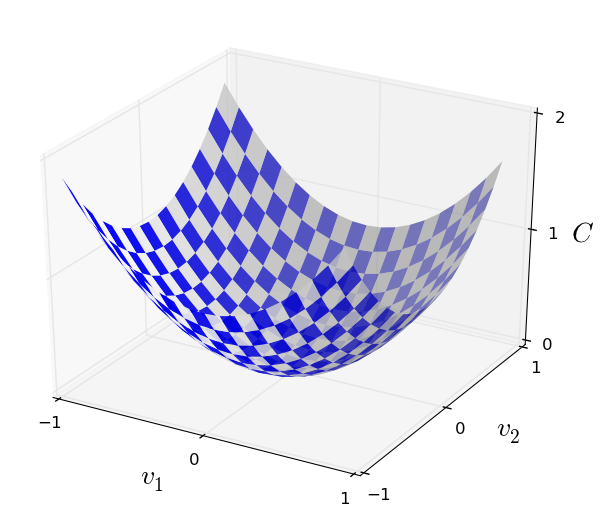
\includegraphics[width=60mm]{valley.png}
  \caption{A 2d convex function as a valley. 
        \href{http://neuralnetworksanddeeplearning.com/chap1.html}{Source}.}
\end{marginfigure}


However, for a class of functions called convex functions, there is a
simple algorithm which is guaranteed to converge to minima. Convex
functions have only one minima. They look something like a valley:

To motivate our algorithm, imagine a ball
is put at a random point on our valley and allowed to roll. Our common
sense tells that ball will eventually roll to the bottom of the valley.

\begin{figure}
  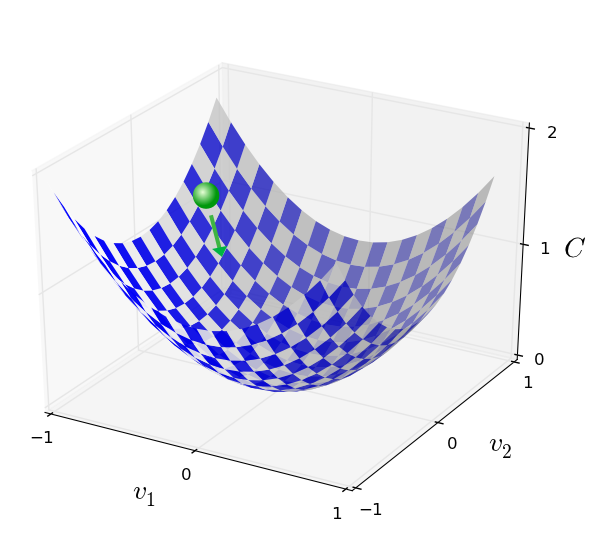
\includegraphics[width=90mm]{valley_with_ball}
  \caption{Gradient descent illustration: a ball on a valley.
\href{http://neuralnetworksanddeeplearning.com/chap1.html}{Source}.}
\end{figure}

Let's roughly simulate the motion of the ball! Key observation is that
the ball moves in the steepest direction of descent. This is negative
\sidenote{Gradient gives us steepest direction of \emph{ascent}.}
of the gradient's direction.

Great! Let's put together our algorithm:

\begin{marginfigure}
  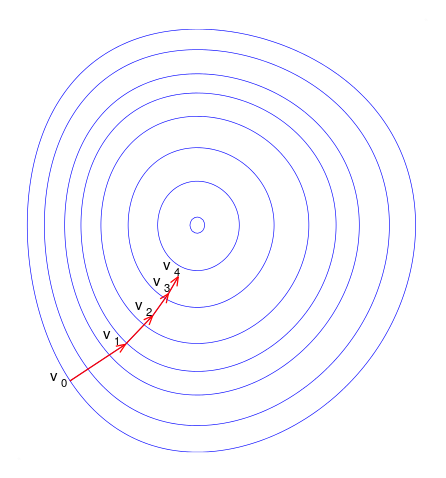
\includegraphics[width=50mm]{Gradient_descent}
  \caption{Gradient descent on a series of level sets.
  \href{https://en.wikipedia.org/wiki/Gradient_descent}{Source}.}
\end{marginfigure}

\begin{algorithm}
\caption{Gradient Descent}
\begin{algorithmic}[1]
  \STATE Start at a random point: \(v\)
  \WHILE{\(v\) hasn't converged}
  \STATE Update \(v\) in the direction of steepest descent: 
      \[v \rightarrow v' = v -\eta \nabla C\]
  \ENDWHILE
\end{algorithmic}
\end{algorithm}



Here \(\eta\) is called \emph{learning rate}. If it is too small,
algorithm can be very slow and might take too many iterations to
converge. If it is too large, algorithm might not even converge.

\subsection{Example: Regression}\label{example-regression}

Let's apply the things learnt above on linear regression problem. Here's
a recap of linear regression:

\begin{quote}
Our model is \(y(x) = wx + b\). Parameters are \(v = (w, b)\) We are
given training pairs \((x^1, y^1), (x^2, y^2), \ldots, (x^n, y^n)\)
\sidenote{ Notation clarifiction: Here, superscripts are indices, not powers }.

We want to find \(w\) and \(b\) which minimize the following cost/loss
function:

\[ C(w, b) = \frac{1}{n} \sum_{i = 1}^{n} C_i(w, b) = \frac{1}{2n} \sum_{i = 1}^{n} \| y(x^i) - y^i\|^2 \]

where
\(C_i(w, b) = \frac{1}{2} \| y(x^i) - y^i\|^2 = \frac{1}{2} \| wx^i + b - y^i\|^2\)
is the loss of the model for \(i\) th training pair.
\end{quote}


Let's calculate gradients,

\[ \nabla C = \frac{1}{n} \sum_{i = 1}^{n} \nabla C_i \]

where \(\nabla C_i\) is computed using:

\[ \nabla C_i = \left( \frac{\partial C_i}{\partial w}, \frac{\partial C_i}{\partial b}  \right) = \left( (wx^i + b - y^i)x^i, (wx^i + b - y^i) \right)\]

Update rule is

\[ v \rightarrow v' = v -\eta \nabla C = v -\frac{\eta}{n} \sum_{i = 1}^{n} \nabla C_i \]


\subsection{Stochastic Gradient Descent}\label{stochastic-gradient-descent}

In the above example, what if we have very large number of samples i.e
\(n \gg 0\)? At every optimization step, we have to compute
\(\nabla C_i\) for each sample \(i = 1, 2, \ldots, n\). This can be very
time consuming!

Can we approximate \(\nabla C\) with a very few samples? Yes!

\[ \nabla C = \frac{1}{n} \sum_{i = 1}^{n} \nabla C_i \approx \frac{1}{m} \sum_{j \in S_m} \nabla C_j \]

where \(S_m\) is random subset of size \(m \ll n\) of
\({1, 2, \ldots,n}\). It turns out that this approximation, even though
estimated only from a small random subset of samples, is good enough for
convergence of gradient descent. This subset of data is called
\emph{minibatch} and this technique is called \emph{stochastic gradient
descent}.

Then stochastic gradient descent works by picking a randomly chosen
subset of data and trains (i.e updates \(v\)) with gradient
approximation computed from them. Next, another subset is picked up and
trained with them. And so on, until we've exhausted all the training
data, which is said to complete an \emph{epoch} of training. Concretely,
following is the stochastic gradient descent algorithm.

\begin{algorithm}
\caption{Stochastic Gradient Descent}
\begin{algorithmic}[1]
  \STATE Start at a random point: \(v\)
  \FOR{a fixed number of epochs}
      \STATE Randomly partition the data into minibatches each of size $m$ 
      \FOR{For each minibatch $S_m$}
        \STATE Update the parameters using \[v \rightarrow v' = v -\frac{\eta}{m} \sum_{i \in S_m} \nabla C_j\]
      \ENDFOR
  \ENDFOR
\end{algorithmic}
\end{algorithm}

\section{Neural Networks}\label{neural-networks}

With this background, we are ready to start with neural networks.

\subsection{Perceptron}\label{perceptron}

Perceptron, a type of artificial neuron was developed in the 1950s and
1960s. Today, it's more common to use Rectified Linear Units (ReLUs).
Nevertheless, it's worth taking time to understand the older models.

So how do perceptrons work? A perceptron takes several inputs,
\(x_1, x_2, \ldots x_n\) and produces a single output:


\begin{figure}
  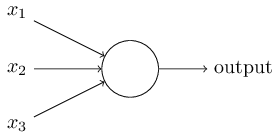
\includegraphics[width=60mm]{tikz0}
  \caption{ Perceptron Model.
\href{http://neuralnetworksanddeeplearning.com/chap1.html}{Source}. }
\end{figure}


\emph{Weights} \(w_1, w_2, \ldots w_n\) decide the importance of each of
the inputs on output \(y(x)\). There is also a \emph{threshold} \(b\) to
decide the output. These are the parameters of the model.
The expression of the output is

\[ y(x) = \sigma\left(\sum_j w_j x_j - b\right) \]

where \(\sigma(z)\) is step function, 

\begin{eqnarray*}
  \sigma(z) & = & \left\{ \begin{array}{ll}
      0 & \mbox{if } z \leq 0 \\
      1 & \mbox{if } z > 0
      \end{array} \right.
\end{eqnarray*}

Therefore 
\begin{eqnarray*}
    y(x) & = & \left\{ \begin{array}{ll}
      0 & \mbox{if } \sum_j w_j x_j \leq b \\
      1 & \mbox{if } \sum_j w_j x_j > b
      \end{array} \right.
\end{eqnarray*}

That's the basic mathematical model. A way you can think about the
perceptron is that it's a device that makes decisions by weighing up
evidence. An example
\sidenote{This example is straight from
\href{http://neuralnetworksanddeeplearning.com/chap1.html}{here}}:

Another way perceptrons can be used is to compute the elementary logical
functions we usually think of as underlying computation, functions such
as \texttt{AND}, \texttt{OR}, and \texttt{NAND}. Check that following
perceptron implements \texttt{NAND}:

\begin{figure}
  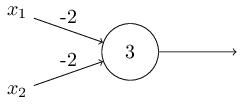
\includegraphics[width=60mm]{tikz2}
  \caption{\texttt{NAND} implemented by perceptron.
\href{http://neuralnetworksanddeeplearning.com/chap1.html}{Source} }
\end{figure}

If you are familiar with digital logic, you will know that \texttt{NAND}
gate is a universal gate. That is, any logical computation can be
computed using just \texttt{NAND} gates. Then, the same property follows
for perceptrons.

\subsection{Multi Layer Perceptrons and Sigmoid}
\label{multi-layer-perceptrons-and-sigmoid}

Although perceptron isn't a complete model of human decision-making, the
above example illustrates how a perceptron can weigh up different kinds
of evidence in order to make decisions. And it should seem plausible
that a complex network of perceptrons could make quite subtle decisions

\begin{figure}
  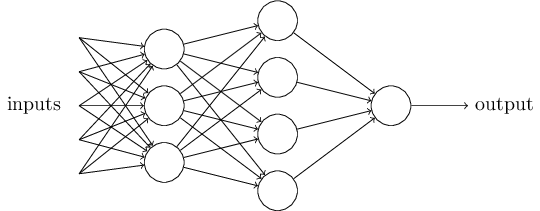
\includegraphics[height=35mm]{tikz1}
  \caption{Multi layer perceptron.
\href{http://neuralnetworksanddeeplearning.com/chap1.html}{Source} }
\end{figure}

This network is called \emph{Multi layered perceptron (MLP)}. In this
MLP, the first column of perceptrons - what we'll call the first
\emph{layer} of perceptrons - is making three very simple decisions, by
weighing the input evidence. What about the perceptrons in the second
layer? Each of those perceptrons is making a decision by weighing up the
results from the first layer of decision-making. In this way a
perceptron in the second layer can make a decision at a more complex and
more abstract level than perceptrons in the first layer. And even more
complex decisions can be made by the perceptron in the third layer. In
this way, a many-layer network of perceptrons can engage in
sophisticated decision making.

How do we learn the parameters of the above model? Gradient Descent!
\sidenote{ MLP model is far from convex.
Therefore, gradient descent is not guaranteed to converge! But it turns
out that it works fine with a few tweaks which we describe below.}
However, the network is very discontinuous. In fact, a small change in
the weights or bias of any single perceptron in the network can
sometimes cause the output of that perceptron to completely flip, say
from 0 to 1. This makes it very difficult for gradient descent to
converge.

How do we overcome this? What is the source of this discontinuity?
Remember that output of perceptron is given by
\(y(x) = \sigma\left(\sum_j w_j x_j - b\right)\) where \(\sigma(z)\) is
step function

\begin{eqnarray*}
  \sigma(z) & = & \left\{ \begin{array}{ll}
      0 & \mbox{if } z \leq 0 \\
      1 & \mbox{if } z > 0
      \end{array} \right.
\end{eqnarray*}

This \(\sigma(z)\) is the source of discontinuity. Can we replace
step function with a smoother version of it?

Check out the following function:

\begin{eqnarray*} 
  \sigma(z) = \frac{1}{1+e^{-z}}.
\end{eqnarray*}

If you graph it, it's quite clear that this function is smoothed out
version of a step function. This function is called \emph{sigmoid}.

\begin{marginfigure}
  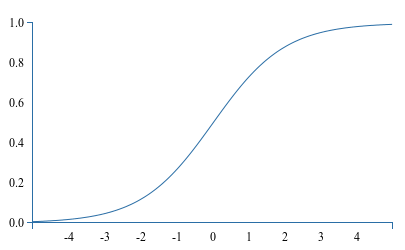
\includegraphics[width=50mm]{sigmoid}
  \caption{Sigmoid function. When \(z\) is large and
  positive, Then \(e^{-z} \approx 0\) and so \(\sigma(z) \approx 1\).
  Suppose on the other hand that \(z\) is very negative. Then
  \(e^{-z} \rightarrow \infty\), and \(\sigma(z) \approx 0\).
  \href{http://neuralnetworksanddeeplearning.com/chap1.html}{Source}.}
\end{marginfigure}

With the \emph{sigmoid neuron}, gradient descent can converges.
Before computing gradients for gradient descent, we need to discuss loss
and activation functions.

\subsection{ReLU Activation}

By now, you have seen that general form of a artificial neuron is
\(y(x) = \sigma\left(\sum_j w_j x_j - b\right)\).
Here the function \(\sigma(z)\) is called \emph{activation
function}. So far, we have seen two different activations:

\begin{enumerate}
\item
  Step function
\item
  Sigmoid function
\end{enumerate}


Let me introduce another activation function, \emph{rectifier} or
\emph{rectified linear unit} (ReLU):

\begin{marginfigure}
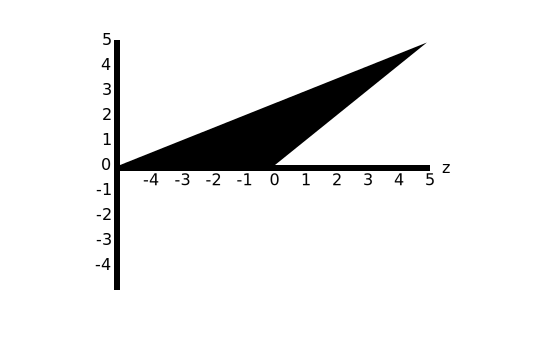
\includegraphics[width=50mm]{relu}
\caption{ ReLU.
\href{http://neuralnetworksanddeeplearning.com/chap3.html}{Source}. }
\end{marginfigure}

\[\sigma(z) = \max(0, z)\]

Because of reasons we describe later
\sidenote{Vanishing gradients problem. Read
more \href{http://neuralnetworksanddeeplearning.com/chap5.html}{here}},
ReLUs are preferred activation functions these days. You will almost
never see sigmoid activation function in modern deep neural networks.

\subsection{Loss functions}

To train any machine learning model, we need to measure who well 
the model fits to training set. This is called loss/cost
\sidenote{I use terms loss function and
cost function interchangeably.} function.
In regression problem we discussed before, cost function was 
\(C(w, b) = \frac{1}{2n} \sum_{i = 1}^{n} \| y(x^i) - y^i\|^2\). 
Minimizing the cost function trains the model.

We will make two assumptions about our cost function:

\begin{enumerate}
\item
  The cost function can be written as an average over cost functions
  \(C_i\) for individual training examples, \((x^i, y^i)\). i.e,
  \(C = \frac{1}{n} \sum_{i = 1}^{n} C_i\)
\item
  Cost can be written as a function of the outputs from the neural
  network. i.e, \(C_i = L(y(x^i), y^i)\) where \(y(x)\) is the output
  from the network.
\end{enumerate}

In the case of regression, we used \(L_2\) loss,
\(L_2(o, y) = \frac{1}{2} \| o - y\|^2\). We could have also used \(L_1\)
loss, \(L_1(o, y) = | o - y |\).

\subsection{Cross Entropy Loss}

What if we have a classification problem? What loss do we use? Consider
a MLP for digit classification on the right.

\begin{marginfigure}
  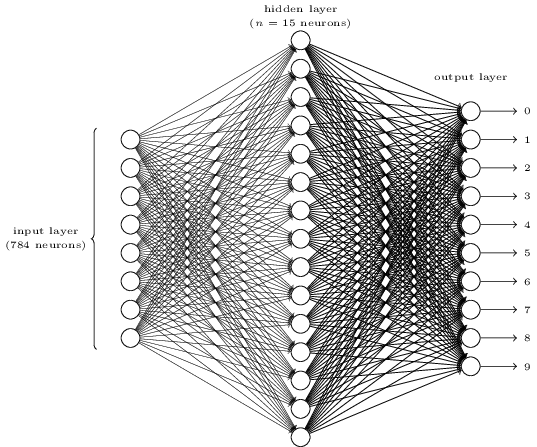
\includegraphics[width=70mm]{tikz12}
  \caption{ MLP for digit classification.
  \href{http://neuralnetworksanddeeplearning.com/chap1.html\%22}{Source}.
  }
\end{marginfigure}

Here, we have output \(o\) of size 10 and a target class \(y\). We could
have used \(L_1(o, e_y)\) or \(L_2(o, e_y)\) loss where \(e_y\) is
\(y\)th unit vector. But it turns out that this doesn't work very well.

Instead, we will consider the outputs as a probability distribution over
10 classes and use what is called a cross entropy loss:

\[ L(o, y) = - \log(o_y) \]

To understand this function, realize that \(o_y\), $y$th output is the predicted
probability of the target class \(y\). Minimizing negative of log of
this probability, maximizes the probability. Also, \(L \geq 0\) because
\(\log(x) < 0\) for \(x \in [0, 1]\).

\subsection{Softmax Activation}

If we use cross entropy loss, we cannot use sigmoids as activations of
output layer because sigmoids do not guarantee a probability
distribution. Although each component of the output will be in \([0, 1]\),
they need not add up to 1.

We therefore use an activation layer called \emph{softmax}. According to
this function, the activation \(a_j\) of the \(j\)th output neuron is

\[ a_j = \frac{e^{z_j}}{\sum_k e^{z_k}} \]

where in the denominator we sum over all the output neurons.
This expression may seem opaque if you are not familiar with it. Observe
the following:

\begin{enumerate}
\item
  Activations are positive: \(a_j \geq 0\)
\item
  Activations sum to 1: \(\sum_j a_j = 1\)
\item
  If you increase \(z_m\) keeping others constant, \(a_m\) increases.
  Other activations decrease to ensure sum remains 1.
\item
  If \(z_m\) is much larger than the others, \(a_m \approx 1\) and
  \(a_k \approx 0\) for \(k \neq m\).
\end{enumerate}

Therefore softmax is a probability distribution which behaves like
smooth version of \texttt{argmax}.

\subsection{Backpropogation}\label{backpropogation}

We have so far discussed the model component of neural networks. We
haven't yet discussed how we learn the parameters of the networks 
i.e, weights and biases of the layers.

As expected, we will use stochastic gradient descent. For this, we need
gradients of \(C_i\), loss for the \(i\)th training example,  
with respect to all the parameters of network. Computation
of this quantity, \(\nabla C_i\) is slightly involved. Let's start with
writing the expression for \(C_i\). Let's represent all the parameters
of the network with \(\theta\):

\[ C_i(\theta) = L\left(y(x^i, \theta), y^i \right)\]

Let's break the above function into composition of layers (or functions
in general)\sidenote{Dropping subscript for brevity}

\[ C = f_L \circ \ f_{L-1} \circ \cdots \circ f_l \circ \cdots \circ f_1 \]

\begin{figure*}
  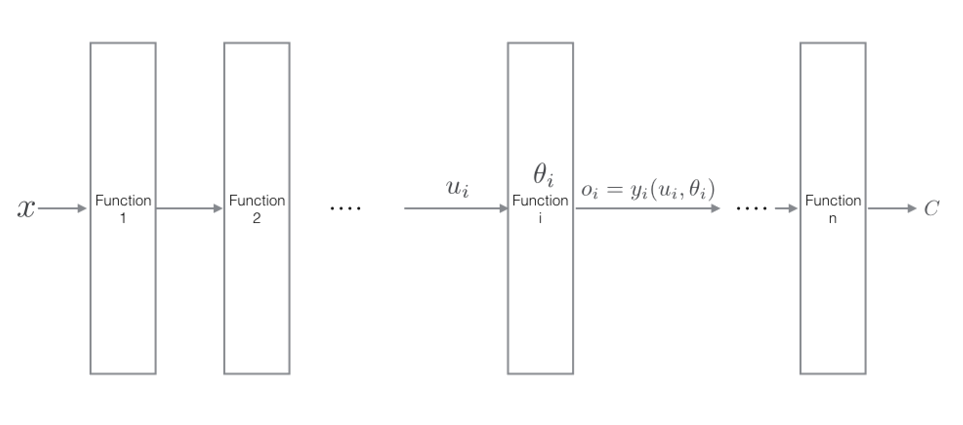
\includegraphics[width=\linewidth]{backprop.png}
  \caption{Cost function as composition}
\end{figure*}


Here, \(l\)th \sidenote{ In particular,
\(C = o_L = f_L(u_L) = L(u_L, y^i)\) } layer/function takes in input
\(u_l\) and outputs \(o_l\)

\begin{equation}
o_l = f_l(u_l, \theta_l) \label{eq:1}
\end{equation}


where \(\theta_l\) are learnable parameters of this layer. Since output
of \(l-1\)th layer is fed to \(l\) th layer as input,


\begin{equation}
u_l = o_{l-1} \label{eq:2}
\end{equation}


We require
\(\nabla C = \left(\frac{\partial C}{\partial\theta_1}, \frac{\partial C}{\partial\theta_2}, \ldots, \frac{\partial C}{\partial\theta_L}\right)\).
Therefore, we need to compute, for  \( l = 1, 2, \dots L \)

\[ \frac{\partial C}{\partial\theta_l} = \frac{\partial o_L}{\partial\theta_l} \]


To compute this quantity, we will compute generic
\sidenote{ You will see ahead why this quantity is useful. }:

\[ \frac{\partial o_m}{\partial \theta_l} \]

Before getting started, let's write down the chain rule. Chain rule is
the underlying operation of our algorithm.

\begin{framed}
\textbf{Chain Rule}: For function f(x, y), 
\begin{equation}
\frac{\partial f}{\partial t} = \frac{\partial f}{\partial x} * \frac{\partial x}{\partial t} + \frac{\partial f}{\partial y} * \frac{\partial y}{\partial t}
\label{eq:3}
\end{equation}

\end{framed}

If \(m > l\),

\begin{equation}
\frac{\partial o_m}{\partial \theta_l} = 0 \label{eq:4}
\end{equation}


because output of the earlier layers doesn't depend on parameters of the later
layer.

If \(m = l\), using equation \eqref{eq:1} and the fact that \(u_l\) and
\(\theta_l\) are independent,

\begin{equation}
\frac{\partial o_l}{\partial \theta_l} = \frac{\partial f_l}{\partial \theta_l}
\label{eq:5}
\end{equation}

\(\frac{\partial f_l}{\partial \theta_l}\) is a computable quantity
which depends on the form of layer \(f_l\).

If \(m < l\), using equation \eqref{eq:1}, \eqref{eq:2}, chain rule \eqref{eq:3},

\begin{align*}
\frac{\partial o_m}{\partial \theta_l} &= \frac{\partial f_m}{\partial \theta_l}\\
&= \frac{\partial f_m}{\partial u_m} * \frac{\partial u_m}{\partial \theta_l} + \frac{\partial f_m}{\partial \theta_m} * \frac{\partial \theta_m}{\partial \theta_l}\\
&= \frac{\partial f_m}{\partial u_m} * \frac{\partial u_m}{\partial \theta_l}\\
&= \frac{\partial f_m}{\partial u_m} * \frac{\partial o_{m-1}}{\partial \theta_l}
\end{align*}


Therefore,

\begin{equation}
\frac{\partial o_m}{\partial \theta_l} = \frac{\partial f_m}{\partial u_m} * \frac{\partial o_{m-1}}{\partial \theta_l}
\label{eq:6}
\end{equation}

Like \(\frac{\partial f_l}{\partial \theta_l}\),
\(\frac{\partial f_l}{\partial u_l}\) is a computable quantity which
depends on layer \(f_l\).

\noindent Let's put everything together and compute the required quantity
\sidenote{Apply \eqref{eq:6} repetitively}:

\begin{align*}
\frac{\partial C}{\partial \theta_l} &= \frac{\partial o_L}{\partial \theta_l}\\
&= \frac{\partial f_L}{\partial u_L} * \frac{\partial o_{L-1}}{\partial \theta_l}\\
&= \frac{\partial f_L}{\partial u_L} * \frac{\partial f_{L-1}}{\partial u_{L-1}} * \frac{\partial o_{L-2}}{\partial \theta_l} \\
&\vdots \\
&= \frac{\partial f_L}{\partial u_L} * \frac{\partial f_{L-1}}{\partial u_{L-1}} * \cdots * \frac{\partial f_{l-1}}{\partial u_{l-1}} * \frac{\partial o_l}{\partial \theta_l}\\
&= \frac{\partial f_L}{\partial u_L} * \frac{\partial f_{L-1}}{\partial u_{L-1}} * \cdots * \frac{\partial f_{l-1}}{\partial u_{l-1}} * \frac{\partial f_l}{\partial \theta_l}
\end{align*}

Now, algorithm to compute gradients \(\nabla C\), i.e.
\(\frac{\partial C}{\partial \theta_l}\) for all \(l\) is fairly clear:

\begin{algorithm}[H]
\caption{Back Propogation}
\begin{algorithmic}[1]
  \STATE \{Forward pass\}
  \STATE Set \(u_0 = x\)
  \FOR {\(l = 1, \dots L\)}
  	\STATE Store \(u_l = f_l(u_{l-1}, \theta_l)\)
  \ENDFOR
  \STATE \{Backward pass\}
  \STATE {Set \(\texttt{buffer} = 1\)}
  \FOR {\(l = L, L-1, \dots 1\)}
  	\STATE Store \(\frac{\partial C}{\partial \theta_l} = \frac{\partial f_l}{\partial \theta_l} * \texttt{buffer}\)
  	\STATE Update \(\texttt{buffer} = \frac{\partial f_l}{\partial u_l} * \texttt{buffer}\)
  \ENDFOR 
  \RETURN \(\left(\frac{\partial C}{\partial\theta_1}, \frac{\partial C}{\partial\theta_2}, \ldots, \frac{\partial C}{\partial\theta_L}\right)\).
\end{algorithmic}
\end{algorithm}


Although this derivation is for scalar functions, it will work with
vector functions with a few modifications.

\subsection{Deep Networks and why they are hard to train}\label{deep-neural-networks}

Whenever you are asked to do any complex task, you usually break it down
to sub tasks and solve the component subtasks. For instance, suppose
you're designing a logical circuit to multiply two numbers. Chances are
your circuit will look something like this:

\begin{figure}
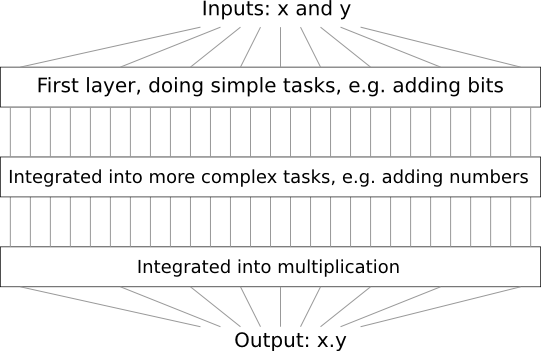
\includegraphics[width=70mm]{circuit_multiplication}
\caption{Logical circuit for multiplication.
\href{http://neuralnetworksanddeeplearning.com/chap5.html\%22}{Source}.
}
\end{figure}

Similarly deep neural networks (i.e lot of layers) can build up multiple
layers of abstraction. Consider the following network:


\begin{figure}
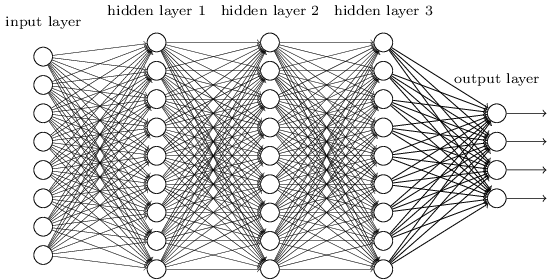
\includegraphics[height=50mm]{tikz36}
\caption{Deep Neural Network.
\href{http://neuralnetworksanddeeplearning.com/chap5.html\%22}{Source}.}
\end{figure}


If we're doing visual pattern recognition, then the neurons in the first
layer might learn to recognize edges, the neurons in the second layer
could learn to recognize more complex shapes, say triangle or
rectangles, built up from edges. The third layer would then recognize
still more complex shapes. And so on. These multiple layers of
abstraction seem likely to give deep networks a compelling advantage in
learning to solve complex pattern recognition problems.

How do we train such deep networks? Stochastic gradient descent as
usual. But we'll run into trouble, with our deep networks not performing
much (if at all) better than shallow networks.
Let's try to understand why are deep networks hard to train:

\begin{enumerate}
\item
  Consider the number of parameters in the network. They are huge! If we
  have to connect 1000 unit hidden layer to 224x224 (50,176) image, we
  have \(65,536*1000 \approx 50e6\) parameters in that layer alone!
  There are so many parameters that network can easily overfit on the
  data without generalization.
\item
  Gradients are unstable. Recall the expression for the gradients,
  \(\frac{\partial C}{\partial \theta_l} = \frac{\partial f_L}{\partial u_L} * \frac{\partial f_{L-1}}{\partial u_{L-1}} * \cdots * \frac{\partial f_{l-1}}{\partial u_{l-1}} * \frac{\partial f_l}{\partial \theta_l}\).
  If few of \(\frac{\partial f_m}{\partial u_m} \ll 1\), they will
  multiply up and make
  \(\frac{\partial C}{\partial \theta_l} \approx 0\)
  \sidenote{ This is the reason why sigmoids are avoided. For sigmoid,
  \(\frac{\partial f}{\partial u} = \frac{d \sigma}{d z}|_{z=u}\) is
  close to zero if \(u\) is either too large or too small. It's maximum
  is only \(1/4\) }. Similarly if few of
  \(\frac{\partial f_m}{\partial u_m} \gg 1\), they make
  \(\frac{\partial C}{\partial \theta_l} \to \infty\). 
\end{enumerate}

Keep these two points in mind. We will see several approaches to deep
learning that to some extent manage to overcome or route around these.


\section{Convolutional Neural
Networks}\label{convolutional-neural-networks}

Let's go back to the problem of handwritten digit recognition. MLP looks
like this:

\begin{figure}
  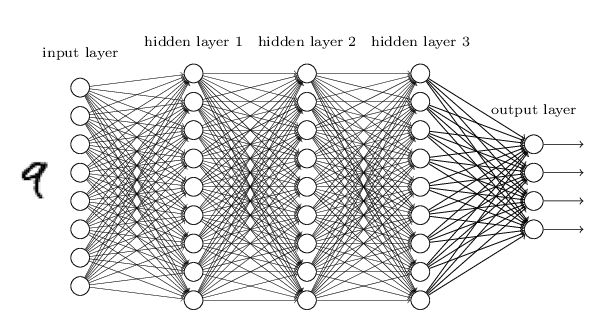
\includegraphics[height=60mm]{mnist_net.png}
  \caption{MLP for MNIST.
  \href{http://neuralnetworksanddeeplearning.com/chap5.html\%22}{Source}.}
\end{figure}


In particular, we have connected all the pixels in 28x28 images i.e, 784
pixels to each neuron in hidden layer 1.

Upon reflection, it's strange to use networks with fully-connected
layers to classify images. The reason is that such a network
architecture does not take into account the spatial structure of the
images. For instance, it treats input pixels which are far apart and
close together on exactly the same footing. Such concepts of spatial
structure must instead be inferred from the training data.

But what if, instead of starting with a network architecture which is
\emph{tabula rasa}, we used an architecture which tries to take
advantage of the spatial structure? In this section I describe
convolutional neural networks. These networks use a special architecture
which is particularly well-adapted to classify images. Using this
architecture makes convolutional networks fast to train. This, in turn,
helps us train deep, many-layer networks, which are very good at
classifying images. Today, deep convolutional networks or some close
variant are used in most neural networks for image recognition.

Convolutional neural networks use three basic ideas:

\begin{enumerate}
\item
  Local receptive fields
\item
  Shared weights
\item
  Pooling.
\end{enumerate}

\subsection{Local receptive fileds}

As per usual, we'll connect the input pixels to a layer of hidden
neurons. But we won't connect every input pixel to every hidden neuron.
Instead, we only make connections in small, localized regions of the
input image.

\begin{figure}
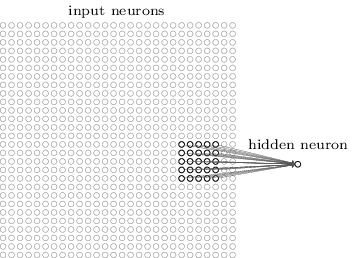
\includegraphics[height=60mm]{conv1}
\caption{Local receptive fields of convolution.
\href{http://neuralnetworksanddeeplearning.com/chap6.html\%22}{Source}.
}
\end{figure}


That region in the input image is called the \emph{local receptive
field} for the hidden neuron. It's a little window on the input pixels.
Each connection learns a weight. And the hidden neuron learns an overall
bias as well. You can think of that particular hidden neuron as learning
to analyze its particular local receptive field.

We then slide the local receptive field across the entire input image.
For each local receptive field, there is a different hidden neuron in
the first hidden layer. To illustrate this concretely, let's start with
a local receptive field in the top-left corner:

\begin{figure}
  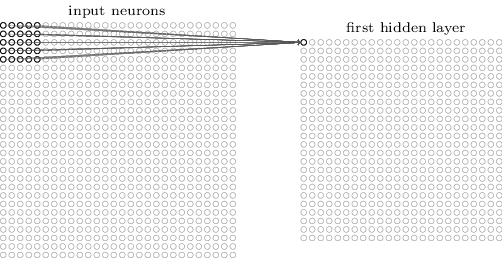
\includegraphics[width=100mm]{conv2}
  \caption{Convolution.
\href{http://neuralnetworksanddeeplearning.com/chap6.html\%22}{Source}.
}
\end{figure}


Then we slide the local receptive field over by one pixel
\sidenote{ Sometimes a different
\emph{stride} length (e.g, 2) is used.} to the right (i.e., by one
neuron), to connect to a second hidden neuron
\sidenote{ Note that if we have a \(28\times 28\) input
image, and \(5\times 5\) local receptive fields, then there will be \(24\times 24\) neurons
in the hidden layer.}:

\begin{figure}
  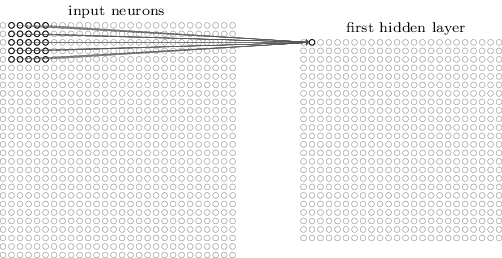
\includegraphics[width=100mm]{conv3}
  \caption{Slide the convolution.
\href{http://neuralnetworksanddeeplearning.com/chap6.html\%22}{Source}.
}
\end{figure}


\subsection{Shared weights and biases}

I've said that each hidden neuron has a bias and 5x5 weights connected
to its local receptive field. What I did not yet mention is that we're
going to use the same weights and bias for each of the 24x24 hidden
neurons.

Sharing weights and biases means that all the neurons in the first
hidden layer detect exactly the same feature just at different locations
in the input image. To see why this makes sense, consider the following
convolution filter:

\begin{figure}
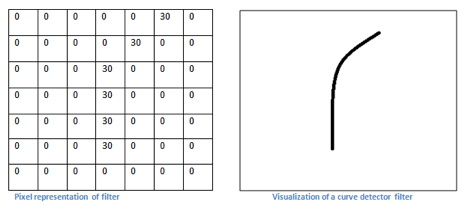
\includegraphics[width=110mm]{conv_example1.png}
\caption{A convolutional filter.
\href{https://adeshpande3.github.io/adeshpande3.github.io/A-Beginner's-Guide-To-Understanding-Convolutional-Neural-Networks/}{Source}.
}
\end{figure}

Let's take an example image and apply convolution on a receptive filed:

\begin{figure}
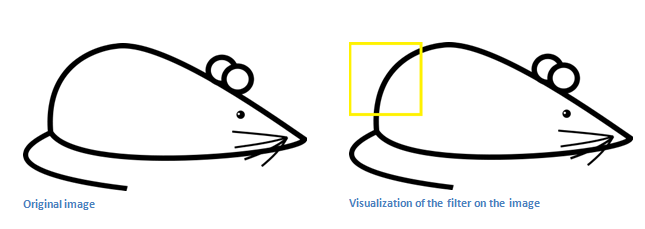
\includegraphics[width=110mm]{conv_example2.png}
\caption{Convolution on an example image.
\href{https://adeshpande3.github.io/adeshpande3.github.io/A-Beginner's-Guide-To-Understanding-Convolutional-Neural-Networks/}{Source}.
}
\end{figure}

\begin{figure}
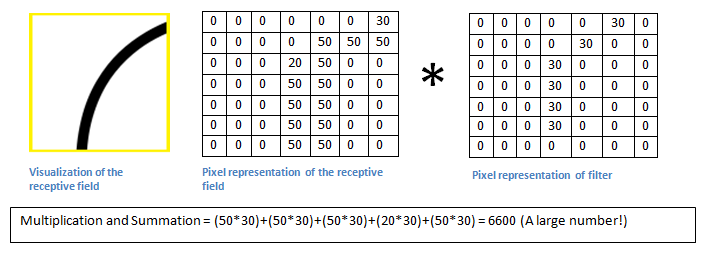
\includegraphics[width=110mm]{conv_example3.png}
\caption{Apply convolution.
\href{https://adeshpande3.github.io/adeshpande3.github.io/A-Beginner's-Guide-To-Understanding-Convolutional-Neural-Networks/}{Source}.
}
\end{figure}

Basically, in the input image, if there is a shape that generally
resembles the curve that this filter is representing, then all of the
multiplications summed together will result in a large value! Now let's
see what happens when we move our filter.

\begin{figure}
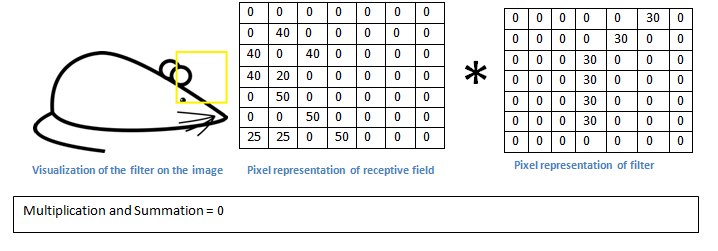
\includegraphics[width=110mm]{conv_example4.png}
\caption{Apply convolution at a different receptive field.
\href{https://adeshpande3.github.io/adeshpande3.github.io/A-Beginner's-Guide-To-Understanding-Convolutional-Neural-Networks/}{Source}.
}
\end{figure}

Therefore, this convolution picks up a right bending curve wherever it
is on . To put it in slightly more abstract terms, convolutional
networks are well adapted to the translation invariance of images: move
a picture of a cat (say) a little ways, and it's still an image of a cat

The network structure I've described so far can detect just a single
kind of localized feature. To do image recognition we'll need more than
one \textbf{feature map}. And so a complete convolutional layer consists
of several different feature maps

\begin{figure}
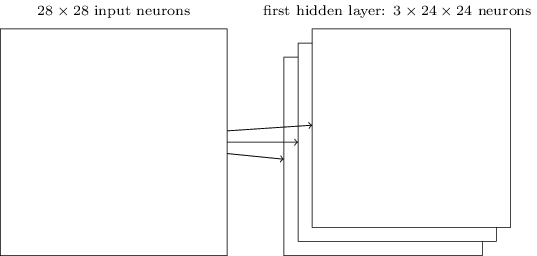
\includegraphics[width=110mm]{conv4.png}
\caption{Apply convolution at a different receptive field.
\href{http://neuralnetworksanddeeplearning.com/chap6.html}{Source}.
}
\end{figure}

A big advantage of sharing weights and biases is that it greatly reduces
the number of parameters involved in a convolutional network. For each
feature map we need 25=5x5 shared weights, plus a single shared bias. So
each feature map requires 26 parameters. If we have 20 feature maps
that's a total of 20x26=520 parameters defining the convolutional layer.
By comparison, suppose we had a fully connected first layer, with
784=28x28 input neurons, and a relatively modest 30 hidden neurons.
That's a total of 784x30 weights, plus an extra 30 biases, for a total
of 23,550 parameters.


\subsection{Pooling layers}

In addition to the convolutional layers just described, convolutional
neural networks also contain pooling layers. Pooling layers are usually
used immediately after convolutional layers. What the \emph{pooling
layers} do is simplify the information in the output from the
convolutional layer.

In detail, a pooling layer takes each feature map output from the
convolutional layer and prepares a condensed feature map. For instance,
each unit in the pooling layer may summarize a region of (say) 2x2
neurons in the previous layer. As a concrete example, one common
procedure for pooling is known as \emph{max-pooling}. In max-pooling, a
pooling unit simply outputs the maximum activation in the 2x2 input
region, as illustrated in the following diagram:

\begin{figure}
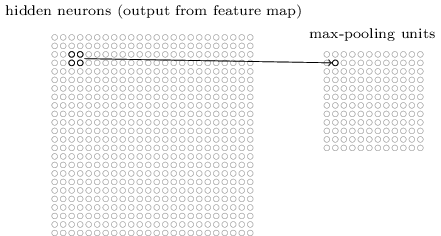
\includegraphics[width=100mm]{max_pooling}
\caption{Pooling Layer.
\href{http://neuralnetworksanddeeplearning.com/chap6.html}{Source}. }
\end{figure}

Note that since we have 24×24 neurons output from the convolutional
layer, after pooling we have 12×12 neurons.

As mentioned above, the convolutional layer usually involves more than a
single feature map. We apply max-pooling to each feature map separately.
So if there were three feature maps, the combined convolutional and
max-pooling layers would look like:

\begin{figure}
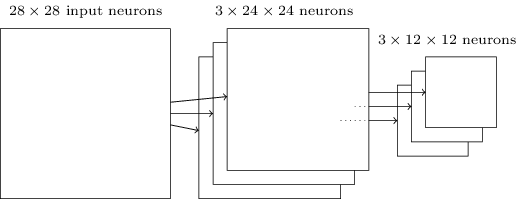
\includegraphics[width=100mm]{max_pooling2}
\caption{Convolution and pooling layer.
\href{http://neuralnetworksanddeeplearning.com/chap6.html}{Source}. }
\end{figure}

We can think of max-pooling as a way for the network to ask whether a
given feature is found anywhere in a region of the image. It then throws
away the exact positional information. The intuition is that once a
feature has been found, its exact location isn't as important as its
rough location relative to other features. A big benefit is that there
are many fewer pooled features, and so this helps reduce the number of
parameters needed in later layers.

\subsection{Case Study: LeNet}\label{case-study-lenet}

Let's put everything we've learnt together and analyze one of the very
early successes \sidenote{LeNet is published in
1998! CNNs are not exactly new.} of convolutional networks: LeNet. This
is the \emph{architecture} of LeNet:

\begin{figure}
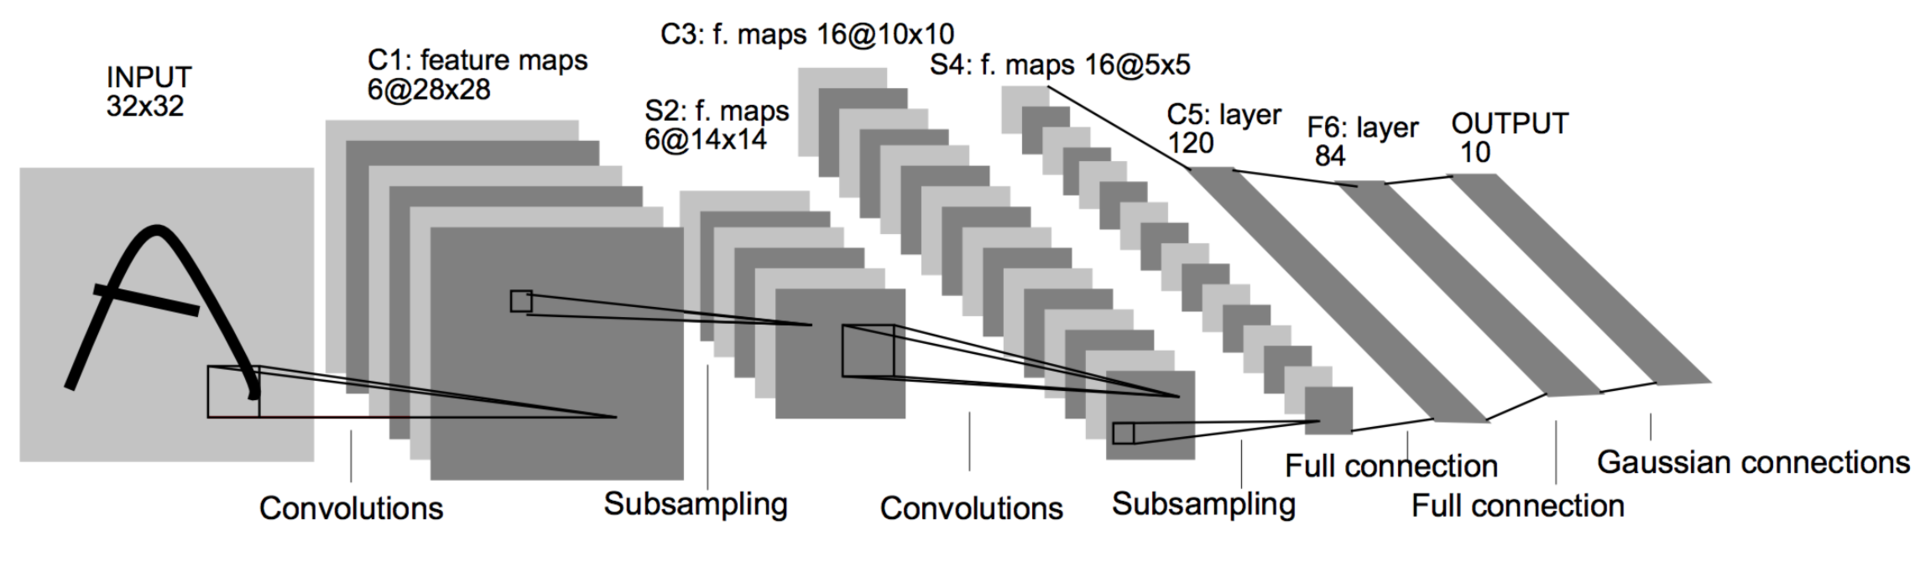
\includegraphics[width=150mm]{lenet.png}
\caption{LeNet architecture
\href{http://yann.lecun.com/exdb/publis/pdf/lecun-01a.pdf}{Source}. }
\end{figure}

Let's go over each of the component layers of LeNet:
\sidenote{ I actually describe slightly modified
version of LeNet. }

\begin{itemize}
\item
  \textbf{Input}: Gray scale image of size 32 x 32.
\item
  \textbf{C1}: Convolutional layer of 6 feature maps, kernel size (5, 5)
  and stride 1. Output size therefore is 6 X 28 x 28. Number of
  trainable parameters is \((5*5 + 1) * 6 = 156\).
\item
  \textbf{S2}: Pooling/subsampling layer with kernel size (2, 2) and
  stride 2. Output size is 6x14x14. Number of trainable parameters =
  0.
\item
  \textbf{C3}: Convolutional layer of 16 feature maps. Each feature map
  is connected to all the 6 feature maps from the previous layer. Kernel
  size and stride are same as before. Output size is 16x10x10.
  Number of trainable parameters is \((6 * 5 * 5 + 1) * 16 = 2416\).
\item
  \textbf{S4}: Pooling layer with same \emph{hyperparameters} as above.
  Output size = 16 x 5 x 5.
\item
  \textbf{C5}: Convolutional layer of 120 feature maps and kernel size
  (5, 5). This amounts to \emph{full connection} with outputs of
  previous layer. Number of parameters are
  \((16 * 5 * 5 + 1)*120 = 48120\).
\item
  \textbf{F6}: \emph{Fully connected layer}\sidenote{This is same as layers in MLP
  we've seen before.} of 84 units. i.e, All units
  in this layer are connected to previous layer's
  outputs. Number of parameters is \((120 + 1)*84 = 10164\)
\item
  \textbf{Output}: Fully connected layer of 10 units with softmax
  activation\sidenote{Ignore `Gaussian connections'.
  It is for a older loss function no longer in use.}.
\end{itemize}

Dataset used was MNIST. It has 60,000 training images and 10,000 testing
examples.

\section{Tricks of the Trade}\label{tricks-of-the-trade}

\subsection{Dropout}\label{dropout}

With so many parameters in neural networks, overfitting is a real
problem. For example, LeNet has about the same number of parameters as
there are training examples. There are a few techniques like
\(L_1\)/\(L_2\) regularization you might be familiar with. These modify
cost function by adding \(L_1\)/\(L_2\) norm of parameters respectively.

Dropout is radically different for regularization. We modify the network
itself instead of the cost function. Suppose we're trying to train a
network:

\begin{figure}
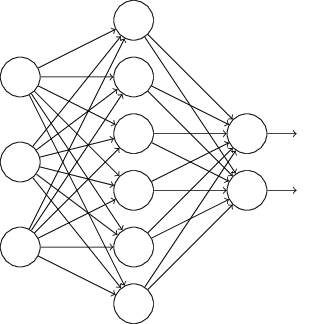
\includegraphics[width=60mm]{dropout1.png}
\end{figure}


With dropout, We start by randomly (and temporarily) deleting half the
hidden neurons in the network, while leaving the input and output
neurons untouched. After doing this, we'll end up with a network along
the following lines.


\begin{figure}
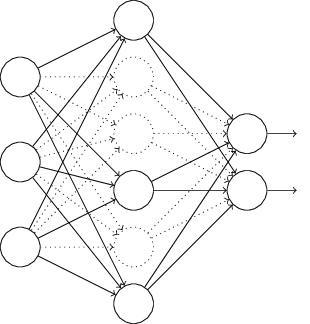
\includegraphics[width=60mm]{dropout2.png}
\end{figure}


We forward-propagate the input \(x\) through the modified network, and
then backpropagate the result, also through the modified network. After
doing this over a mini-batch of examples, we update the appropriate
weights and biases. We then repeat the process, first restoring the
dropout neurons, then choosing a new random subset of hidden neurons to
delete, estimating the gradient for a different mini-batch, and updating
the weights and biases in the network.

The weights and biases will have been learnt under conditions in which
half the hidden neurons were dropped out. When we actually run the full
network that means that twice as many hidden neurons will be active. To
compensate for that, we halve the weights outgoing from the hidden
neurons.

Why would dropout help? Explanation from
\href{https://papers.nips.cc/paper/4824-imagenet-classification-with-deep-convolutional-neural-networks.pdf}{AlexNet}
paper \sidenote{AlexNet is the paper which lead
to renaissance of CNNs.}:

\begin{quote}
This technique reduces complex co-adaptations of neurons, since a neuron
cannot rely on the presence of particular other neurons. It is,
therefore, forced to learn more robust features that are useful in
conjunction with many different random subsets of the other neurons.
\end{quote}

In other words, we can think of dropout as a way of making sure that the
model is robust to the loss of any individual piece of evidence. Of
course, the true measure of dropout is that it has been very successful
in improving the performance of neural networks.

\subsection{Data Augmentation}\label{data-augmentation}

You probably already know that more data leads to better accuracy. It's
not surprising that this is the case, since less training data means our
network will be exposed to fewer variations in the way human beings
write digits.

Obtaining more training data can be expensive, and so is not always
possible in practice. However, there's another idea which can work
nearly as well, and that's to artificially expand the training data.
Suppose, for example, that we take an MNIST training image of a five,

\begin{figure}
  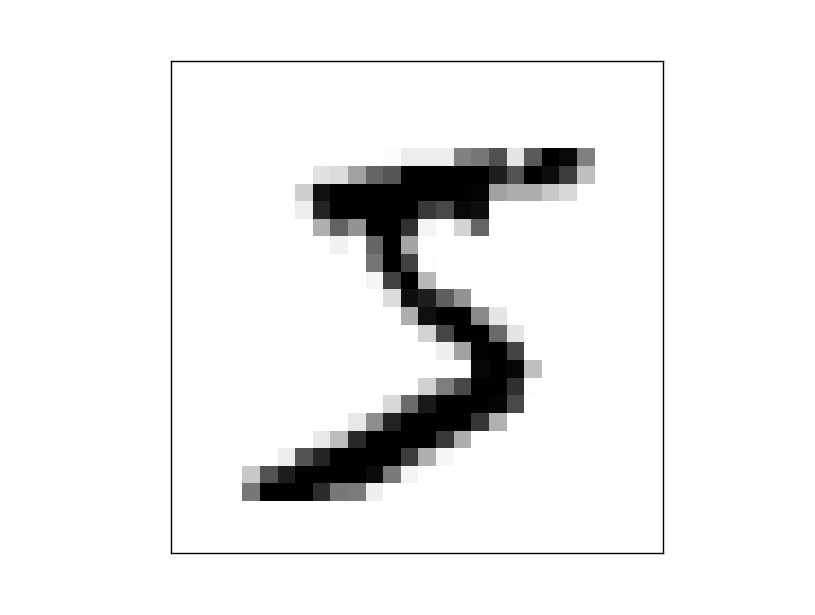
\includegraphics[width=30mm]{more_data_5.png}
\end{figure}

and rotate it by a small amount, let's say 15 degrees:

\begin{figure}
  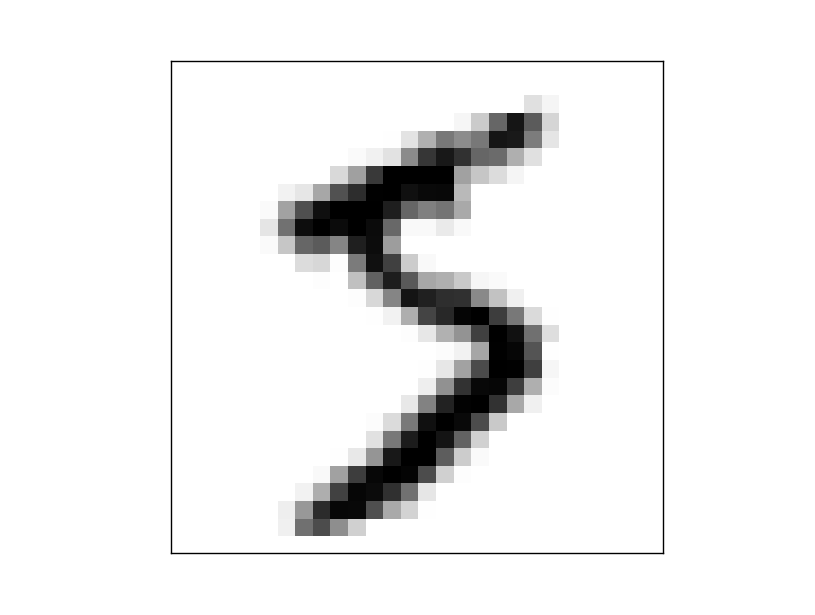
\includegraphics[width=30mm]{more_data_rotated_5.png}
\end{figure}


It's still recognizably the same digit. And yet at the pixel level it's
quite different to any image currently in the MNIST training data. We
can expand our training data by making \emph{many} small rotations of
all the MNIST training images, and then using the expanded training data
to improve our network's performance.

We call such expansion as \emph{data augmentation}. Rotation is not the
only way to augment the data. A few examples are crop, zoom etc. The
general principle is to expand the training data by applying operations
that reflect real-world variation.

\subsection{Weight initialization and Batch
Normalization}\label{weight-initialization-and-batch-normalization}

Training a neural network is a highly non convex problem. Therefore,
initialization of parameters to be optimized is important. To understand
better, recall the unstable gradient problem. This is the equation of
gradients for parameters in \(j\)th layer:

\[\frac{\partial C}{\partial \theta_l} = \frac{\partial f_L}{\partial u_L} * \frac{\partial f_{L-1}}{\partial u_{L-1}} * \cdots * \frac{\partial f_{l-1}}{\partial u_{l-1}} * \frac{\partial f_l}{\partial \theta_l}\]

If a layer is not properly initialized, it scales inputs by \(k\), i.e
\(\frac{\partial f_m}{\partial u_m} \approx k\). Therefore gradients of
parameters in \(l\) th layer is

\[\frac{\partial C}{\partial \theta_l} = k^{L - l}\]

Thus, \(k > 1\) leads to extremely large gradients and \(k<1\) to very
small gradients in initial layers. Therefore, we want

\[k \approx 1\]

This can be made sure with good weight initialization. Historically, bad
weight inits are what prevented deep neural networks to be trained.

A recently developed technique called
\href{http://arxiv.org/abs/1502.03167}{Batch Normalization} alleviates a
lot of headaches with initializations by explicitly forcing this
throughout a network. The core observation is that this is possible
because normalization is a simple differentiable operation.

It has become a very common practice to use Batch Normalization in
neural networks. In practice, networks that use Batch Normalization are
significantly more robust to bad initialization.

\section{Practical Advice}\label{practical-advice}

\subsection{ImageNet Dataset and
ILSVRC}\label{imagenet-dataset-and-ilsvrc}

ImageNet is a \emph{huge} dataset for visual recognition research. It
currently has about \emph{14 million} images tagged manually.

ImageNet project runs an annual contest, the ImageNet Large
Scale Visual Recognition Challenge (ILSVRC), where algorithms compete
 to correctly classify and detect objects and scenes. ILSVRC
recognition challenge is conducted on a subset of ImageNet: 1.2 million
images with 1000 classes.

Here are example images and the recognition results:
\begin{figure}
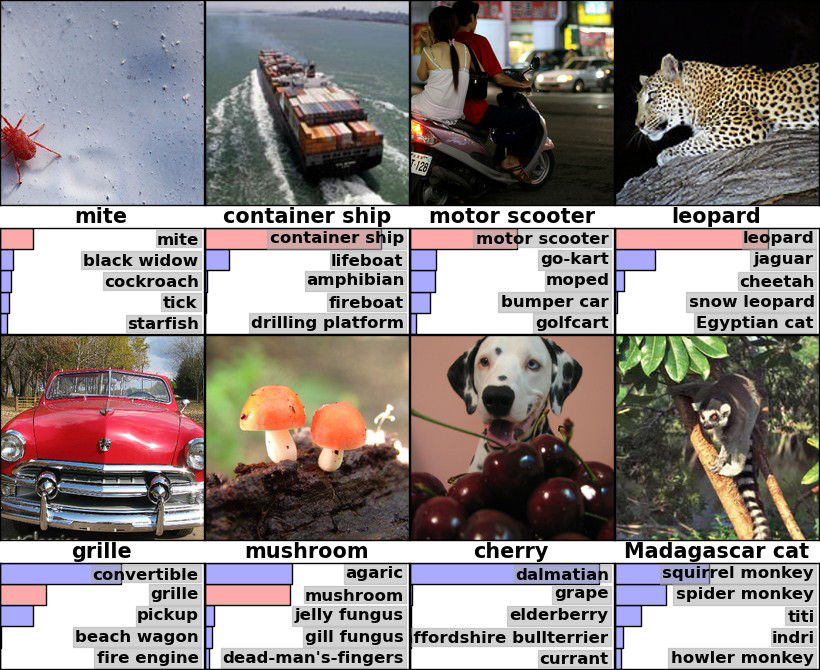
\includegraphics[width=110mm]{imagenet.png}
\caption{Images from imagenet.
\href{http://mappingignorance.org/fx/media/2013/04/Deep-learning-5.png}{Source}.
}  
\end{figure}


\href{https://papers.nips.cc/paper/4824-imagenet-classification-with-deep-convolutional-neural-networks.pdf}{Alexnet}
was the first CNN to participate in ILSVRC and won the 2012 challenge by
a significant margin. This lead to a renaissance of CNNs for visual
recognition. This is the architecture:
\begin{figure}
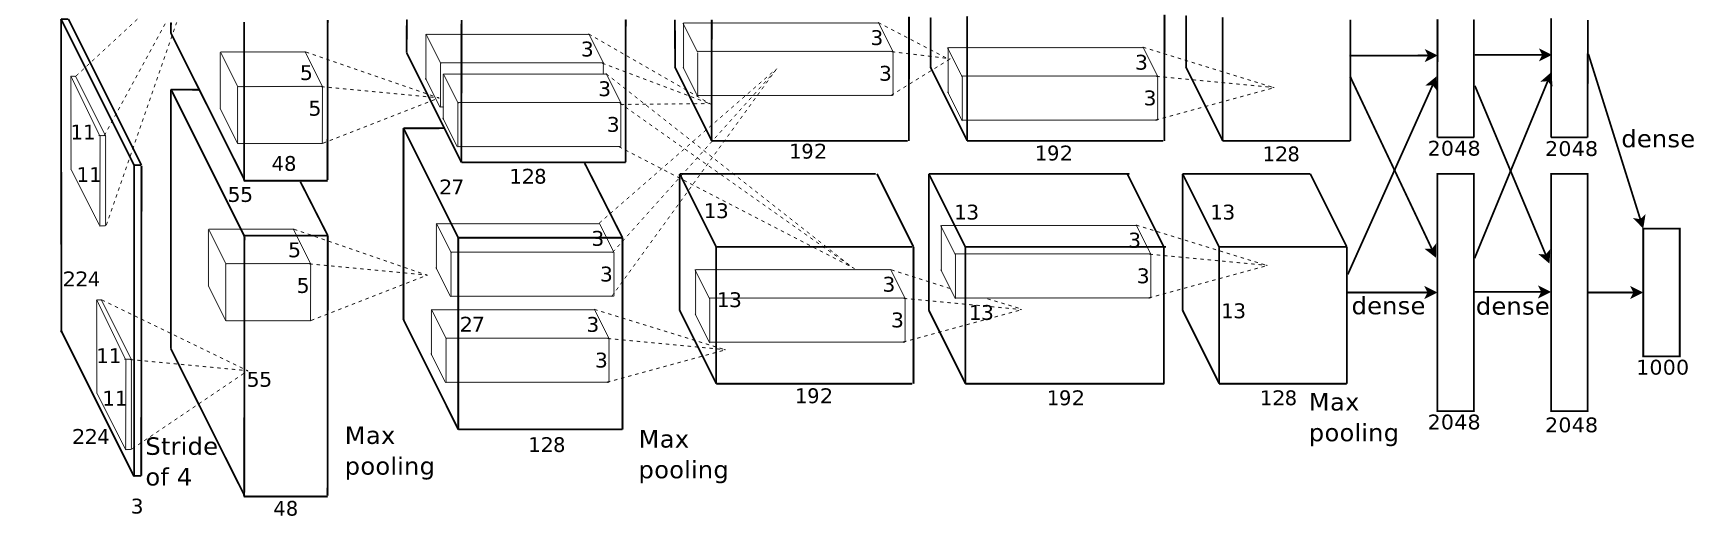
\includegraphics[width=110mm]{alexnet.png}
\caption{Alexnet architecture.
\href{http://mappingignorance.org/fx/media/2013/04/Deep-learning-5.png}{Source}.
}  
\end{figure}


It isn't too different from LeNet we discussed before. Over the years,
newer CNN architectures won this challenge. Notable ones are

\begin{itemize}
\item
  \href{https://arxiv.org/pdf/1409.1556}{VGGNet}
\item
  \href{https://research.google.com/pubs/pub43022.html}{GoogLeNet}
\item
  Inception
\item
  \href{https://arxiv.org/abs/1512.03385}{ResNet}
\end{itemize}

You will keep on hearing these architectures if you work more on CNNs. Here
are the accuracies from these networks:

\begin{figure}
  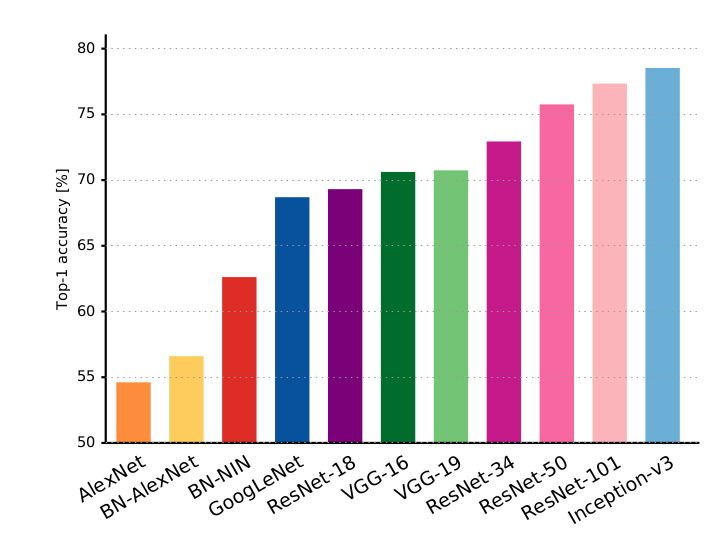
\includegraphics[width=70mm]{imagenet-top1.png}
  \caption{Top 1 accuracies on ILSVRC.
\href{https://chaosmail.github.io/deeplearning/2016/10/22/intro-to-deep-learning-for-computer-vision/\#Canziani16}{Source}.
}
\end{figure}

\subsection{Transfer Learning}\label{transfer-learning}

To train a CNNs like above from scratch (i.e random initialization), you
will need a huge dataset of the ImageNet scale. In practice, very few
people do this.

Instead, you will pretrain your network on large dataset like imagenet
and use the learned weights as initializations. Usually, you will just
download the trained model of one of the above architectures from
internet and use them as your weight initializations. This is called
\emph{transfer learning}.

This is a very powerful trick. For example,
\href{http://pytorch.org/tutorials/beginner/transfer_learning_tutorial.html}{here}
pretrained weights of ResNet-18 are used to train a classifier to
classify ants and bees.

\begin{figure}
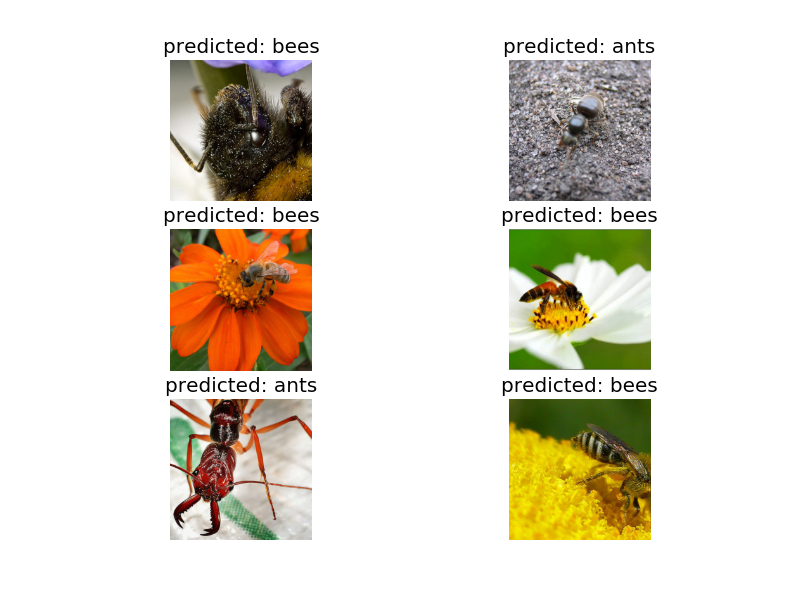
\includegraphics[width=110mm]{transfer_learning.png}
\caption{Ants/Bees classifier.
\href{http://pytorch.org/tutorials/beginner/transfer_learning_tutorial.html}{Source}.
}  
\end{figure}

This is the dataset used:
\begin{description}
\item[Training]: 120 ants + 120 bees images
\item[Testing]: 75 ants + 75 bees images
\end{description}

With this small dataset, accuracy is around 95 \% !

Why does transfer learning work? 1.2 million images in imagenet cover
wide diversity of real world images. Filters learned on imagenet will
therefore be sufficiently general to apply on any similar problem. i.e,
you will not overfit on your small dataset.

Moral of the story: you don't need a large dataset if you are working on
real life images!

\subsection{GPUs}\label{gpus}

GPUs dramatically speed up neural networks. This is because most of the
neural network computation is just matrix multiplication and thus is
readily vectorizable. GPUs excel at such computations.

For example, look at the times taken by the above transfer learning code to
train:

\begin{description}
\item[CPU]: \textasciitilde{} 20 min
\item[GPU]: \textasciitilde{} 1 min
\end{description}

And this was with meager dataset of 400 images. Imagine working with a
dataset of the scale of ImageNet. GPUs are essential if you are serious
about deep learning.

\subsection{Other FAQ}\label{other-faq}

\noindent What framework to use?

\begin{quote}
Lot of frameworks are available: Keras, Tensorflow, PyTorch. I suggest
using Keras if you are new to deep learning.
\end{quote}

\noindent How do I know what architecture to use?

\begin{quote}
Don't be a hero!

\begin{itemize}
\item
  Take whatever works best on ILSVRC (latest ResNet)
\item
  Download a pretrained model
\item
  Potentially add/delete some parts of it
\item
  Finetune it on your application.
\end{itemize}
\end{quote}

\noindent How do I know what hyperparameters to use?

\begin{quote}
Don't be a hero!

\begin{itemize}
\item
  Use whatever is reported to work best on ILSVRC.
\item
  Play with the regularization strength (dropout rates)
\end{itemize}
\end{quote}

\noindent But my model is not converging!

\begin{quote}
\begin{itemize}
\item
  Take a very small subset (like, 50 samples) of your dataset and train
  your network on this.
\item
  Your network should completely overfit on this data. If not play with
  learning rates. If you couldn't get your network to overfit, something
  is either wrong with your code/initializations or you need to pick a
  more powerful model.
\end{itemize}
\end{quote}


\end{document}
